\chapter{Analisis dan Perancangan}
\label{chap:Analisis dan Perancangan}

Pada bab ini, penulis akan menjelaskan apa saja yang dilakukan dalam pengembangan \textit{Agglomerative Hierarchical Clustering} untuk Spark. Pengembangan dilakukan untuk mencapai tujuan yaitu mendapatkan pola dari dataset yang diolah. Pola yang ingin didapatkan meliputi perhitungan rata-rata, nilai maksimum, nilai minimum dan nilai standar deviasi dari setiap atribut yang ada pada data. Selain itu, perlu didapatkan juga jumlah anggota pada setiap \textit{cluster} yang dihasilkan dari algoritma \textit{Hierarchical Agglomerative Clustering}.


\section{Analisis Masalah}

Pada bagian ini akan dijelaskan masalah dari penelitian ini, analisis algoritma \textit{Hierarchical Agglomerative Clustering} dan analisis masukan. 

\subsection{Identifikasi Masalah}

Dalam bidang \textit{big data}, volume data yang sangat besar harus disimpan dalam tempat penyimpanan yang sangat besar. Volume data \textit{big data} dapat mencapai \textit{peta bytes}. Volume yang terlalu besar akan meningkatkan biaya dan menghabiskan tempat penyimpanan data. Volume data perlu direduksi agar menghemat tempat dan biaya.\\ 

Teknologi Hadoop MapReduce dan algoritma \textit{Agglomerative Hierarchical Clustering} dapat digabungkan sebagai solusi untuk mereduksi data. Algoritma \textit{Agglomerative} dapat mereduksi data dengan mengambil pola-pola dari \textit{clusters} yang dibentuk. Sistem terdistribusi Hadoop membantu dalam proses membagikan dan memecah tugas agar dapat dikerjakan secara paralel.  Dengan begitu, proses reduksi data dengan algoritma \textit{Agglomerative} akan lebih cepat. \\

Tetapi teknologi Hadoop masih terlalu lambat dalam mereduksi data. Hal ini disebabkan karena Hadoop banyak melakukan penulisan dan pembacaan kepada disk. Proses \textit{disk} I/O pada Hadoop sangat tinggi dan menyebabkan algoritma \textit{Agglomerative} berjalan sangat lambat pada Hadoop. Pada setiap tahap Hadoop akan menuliskan hasilnya kepada \textit{disk} dan akan dibaca kembali oleh tahap selanjutnya dari \textit{disk} seperti pada Gambar  ~\ref{fig:mapreducediagram}.\\

\begin{figure}[H]
    \centering  
    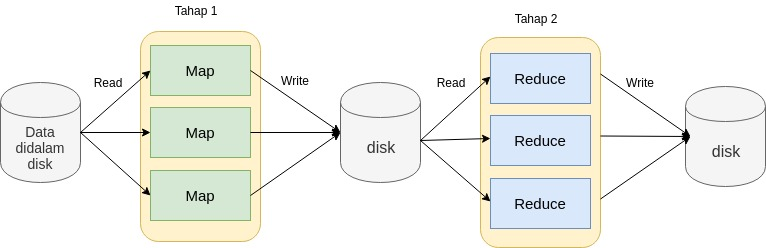
\includegraphics[scale=0.5]{mapreducediagram}  
    \caption[Penulisan kepada disk di MapReduce]{Penulisan kepada disk di MapReduce} 
    \label{fig:mapreducediagram} 
\end{figure}


Solusinya adalah menggabungkan teknologi terdistribusi lainnya dengan  algoritma \textit{Agglomerative} untuk mereduksi data. Spark, sistem terdistribusi yang menyimpan data pada memori dapat menggantikan Hadoop MapReduce. Kecepatan memori lebih cepat dibanding disk merupakan salah satu faktor mengapa Spark akan memproses data dengan kecepatan yang lebih tinggi.  Pembacaan han penulisan akan dilakukan kepada memori. Gambar ~\ref{fig:memorydiagram} adalah contoh ilustrasi tahap proses data di Spark. 
	
\begin{figure}[H]
    \centering  
    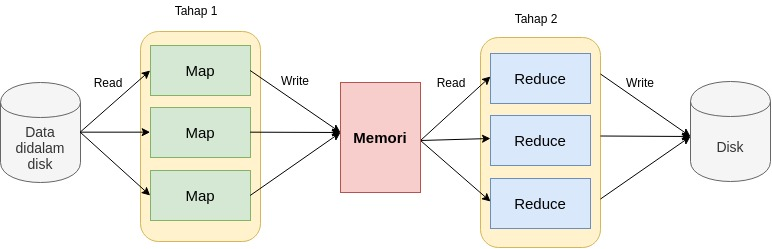
\includegraphics[scale=0.5]{memorydiagram}  
    \caption[Penulisan kepada memori di Spark]{Penulisan kepada memori di Spark} 
    \label{fig:memorydiagram} 
\end{figure}

 
\subsection{Analisis Hierarchical Agglomerative Clustering MapReduce}

Sebelum melakukan perancangan, penulis terlebih dahulu mempelajari algoritma \textit{Hierarchical Agglomerative Clustering} pada Hadoop. Algoritma \textit{Hierarchical Agglomerative Clustering}  pada MapReduce dibagi menjadi dua bagian. Bagian pertama terkait tahap \textit{map} dan bagian kedua terkait tahap \textit{reduce}. Tahap map bertujuan untuk membagi rata data menjadi beberapa partisi agar setiap \textit{reducer} mendapatkan pekerjaan yang hampir rata dengan \textit{reducer} yang lainya. Tahap \textit{map} akan dijelaskan dengan \textit{pseudocode} berikut ini \ref{alg:mapper}:\\

\begin{algorithm}[H]
	\DontPrintSemicolon\SetAlgoNoLine\LinesNumbered
	\SetKwInOut{Input}{Masukan}
	\SetKwInOut{Output}{Keluaran}
	\SetKwInOut{Desc}{Deskripsi}
	\Input{Data mentah (\textbf{TO}), jumlah partisi (\textbf{$n$}) }
	\Output{\textit{key} = sebuah bilangan bulat $\epsilon$ \{1 ... \textbf{$n$}\}, \textit{value} = teks dari sekumpulan nilai atribut yang telah diproses sebelumnya}
	\Desc{memecah \textbf{TO} dengan memberi bilangan acak untuk setiap objek}
	\BlankLine
	\SetKwHangingKw{va}{\textbf{value} $\leftarrow$}
	\SetKwHangingKw{ke}{\textbf{key} $\leftarrow$}
	\SetKwHangingKw{hasil}{}
	\Begin{
		\va{membaca baris  dan memproses atributnya}
		\ke{sebuah bilangan acak $k$, dimana 1 $\leq$ $k$ $\leq$ $n$ }
		mengembalikan pasangan <\textit{key}, \textit{value}> sebagai hasil
	}
	
	
	\caption{Algoritma \textit{Mapper}}
	\label{alg:mapper}
\end{algorithm}

Tahap \textit{reduce} bertujuan untuk mereduksi data. Pada tahap ini dendrogram akan dibangun dari hasil tahap \textit{map}. Setelah membangun \textit{dendrogram}, \textit{dendrogram} akan dipotong untuk menghasilkan \textit{clusters}. Kemudian, pola akan dihitung dari \textit{clusters} dan disimpan kepada file. Tahap \textit{reduce} akan dijelaskan dengan \textit{pseudocode} berikut ini \ref{alg:reducer}:\\

\begin{algorithm}[H]
	\DontPrintSemicolon\SetAlgoNoLine\LinesNumbered
	\SetKwInOut{Input}{Masukan}
	\SetKwInOut{Output}{Keluaran}
	\SetKwInOut{Desc}{Deskripsi}
	\Input{pasangan <\textit{key},\textit{value}> dari mapper dimana semua \textit{value}-nya memiliki nilai \textit{key} yang sama, \textit{maxObject}, \textit{distType}  $\epsilon$ \{\textit{single}, \textit{complete}, \textit{means}\}, \textit{cut-off distance} \{$co$\} }
	\Output{pola \textit{cluster}, $c$}
	\Desc{Membuat \textit{dendrogram} dari hasil \textit{map} sesuai dengan batasan yang diberikan, membatasi jumlah objek yang akan diolah menjadi \textit{dendrogram} berdasarkan \textit{maxObject}, menghitung pola dari \textit{cluster} berdasarkan nilai $co$, menuliskan hasil pola kepada file }
	\BlankLine
	\SetKwHangingKw{ls}{\textbf{\textit{listTrees}} $\leftarrow$ []}
	\SetKwHangingKw{node}{\textbf{\textit{node}} $\leftarrow$}
	\SetKwHangingKw{isFalse}{\textbf{\textit{isProcessed}} $\leftarrow$}
	\SetKwHangingKw{isTrue}{\textbf{\textit{isProcessed}} $\leftarrow$}
	\Begin{
	\ls{}
		\ForEach{pasangan <\textit{key}, \textit{value>}}{
				\node{\textit{value}}
				tambahkan \textbf{\textit{node}} kepada \textbf{listTrees}\;
				\isFalse{false}
				\If{\textbf{listTrees}.length == maxObject}{
					bangun dendrogram dari \textbf{listTress} berdasarkan tipe \textit{distType}\;
					bentuk \textit{clusters} dari dendrogram bedasrkan nilai \textit{co}\;
					hitung pola $c$ dari setiap \textit{cluster} yang dibentuk dan simpan hasil kepada file\;
					kosongkan \textbf{listTress}\;
					\isFalse{True}
				}
			
		}
		\If{isProcessed == false}{
			bangun dendrogram dari \textbf{listTress} berdasarkan tipe \textit{distType}\;
			bentuk \textit{clusters} dari dendrogram bedasrkan nilai \textit{co}\;
			hitung pola $c$ dari setiap \textit{cluster} yang dibentuk dan simpan hasil kepada file\;
		}
	}
	
	
	\caption{Algoritma \textit{reducer}}
	\label{alg:reducer}
\end{algorithm}

\subsection{Analisis Masukan dan Keluaran}

Dalam melakukan perancangan perlu diketahui dulu kebutuhan perangkat lunak. Perangkat lunak yang dirancang harus dapat menangani \textit{input} yang diberikan seperti contoh dibawah. Setiap baris mewakili sebuah objek beserta atributnya. Atribut dipisahkan dengan tanda koma. Setiap atribut merupakan bilangan desimal. Setiap objek dapat memiliki lebih dari satu atribut.

\begin{verbatim}
97.92268076905681,95.67804892782392
15.875897725375477,81.36427207827654
15.825886365695096,6.163384415958262
69.28295038155534,85.36655250595662
10.032110782002924,98.13534474918522
38.53402755308164,96.99987611939603
45.17834148867077,5.96338806209017
91.66074344459808,15.182927773314525
....
....
\end{verbatim} 

Selain itu, perangkat lunak harus dapat menghasilkan pola seperti berikut:

\begin{enumerate}

\item Jumlah objek pada \textit{cluster}.

\item Nilai minimum setiap atribut pada \textit{cluster}.

\item Nilai maksimum setiap atribut pada \textit{cluster}.

\item Nilai rata-rata setiap atribut pada \textit{cluster}.

\item Nilai standar deviasi setiap atribut pada \textit{cluster}.
\end{enumerate}

\subsection{Diagram Alur}

\begin{figure}[H]
    \centering  
    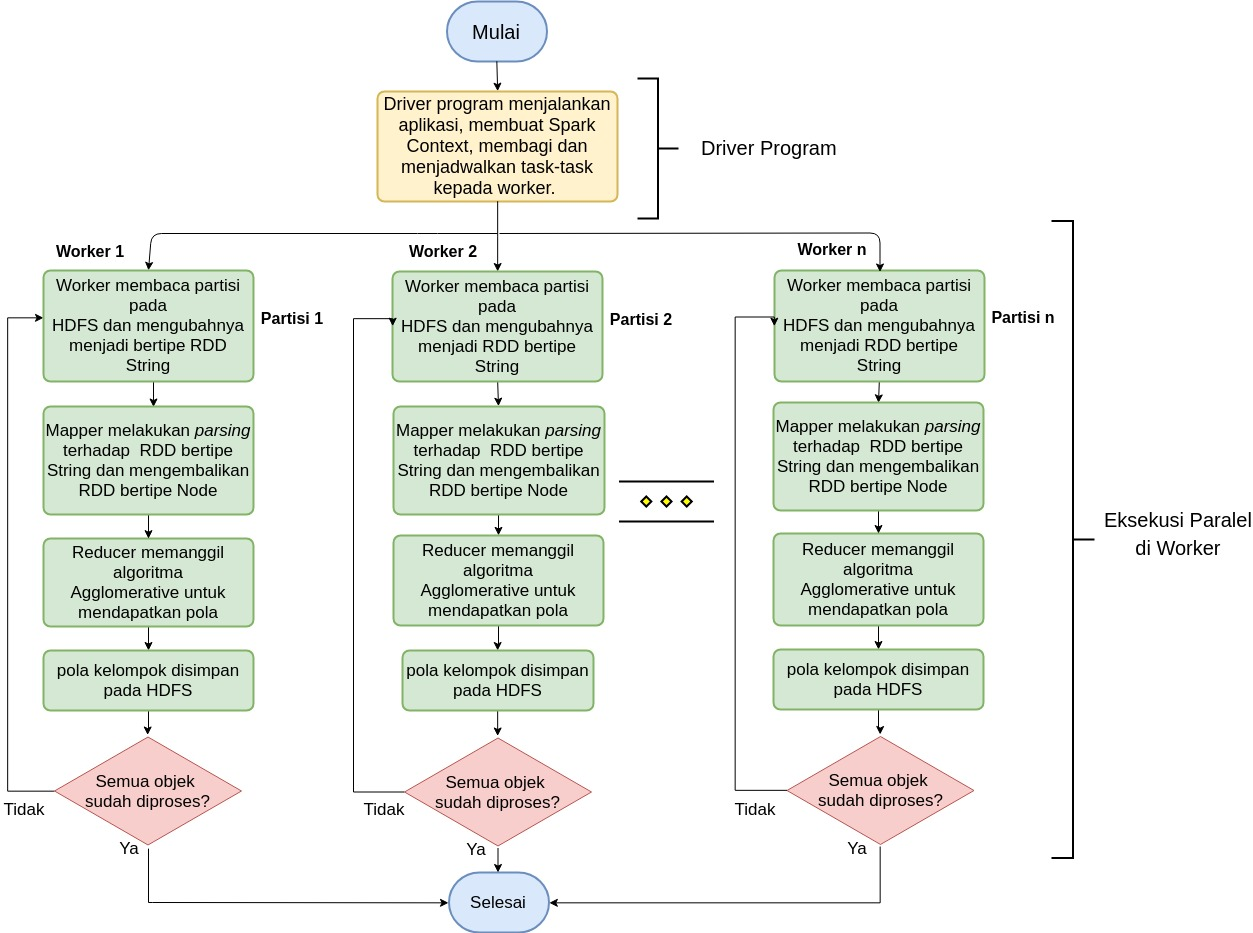
\includegraphics[scale=0.4]{flowc}  
    \caption[Diagram alur perangkat lunak]{Diagram alur perangkat lunak} 
    \label{fig:flowc} 
\end{figure}

Diagram alur diatas (Gambar ~\ref{fig:flowc}) digunakan untuk menjelaskan alur perangkat lunak. Berikut adalah penjelasan alur perangkat lunak:

\begin{enumerate}

\item Pertama-tama aplikasi akan dijalankan pada \textit{driver program}. Kemudian \it{Spark Context} akan dibuat dan operasi-operasi pada aplikasi diubah menjadi \it{task-task}. \it{Task-task} tersebut akan dibagikan dan dijadwalkan kepada \it{worker} oleh \it{driver program}. 


\item Kemudian, \it{worker} akan membaca partisi HDFS yang ditentukan oleh \it{driver program}. Worker akan mengubah file-file tersebut menjadi RDD bertipe String seperti pada Gambar ~\ref{fig:rddpartition}.

\begin{figure}[H]
    \centering  
    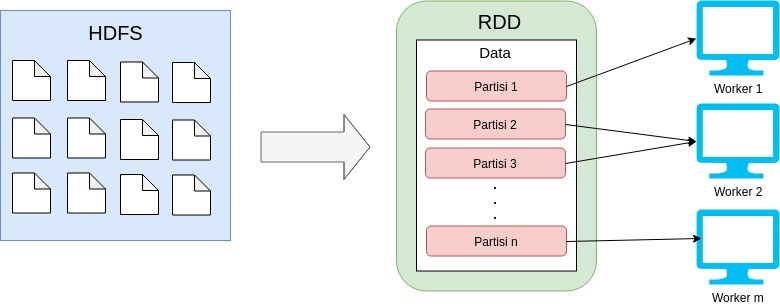
\includegraphics[scale=0.5]{rddpartition}  
    \caption[Partisi RDD]{Partisi RDD} 
    \label{fig:rddpartition} 
\end{figure}

\item Selanjutnya, partisi yang mengandung RDD bertipe \it{String} akan di-\it{parsing}. Objek dalam RDD bertipe \it{String} akan diubah menjadi objek \it{Node} seperti pada Gambar~\ref{fig:mapperspark}. Dari tahap ini akan dihasilkan RDD berisi objek-objek \it{Node}. Worker akan memproses setiap partisi sampai seperti pada Gambar~\ref{fig:workerprocess}.

\begin{figure}[H]
    \centering  
    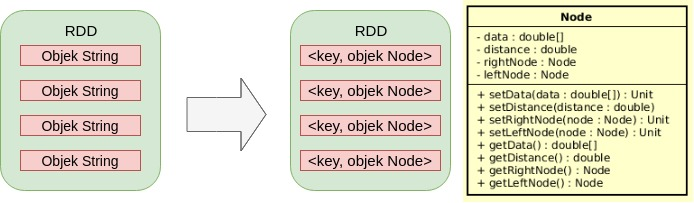
\includegraphics[scale=0.6]{mapperspark}  
    \caption[RDD \textit{parsing} dan kelas \textit{Node}]{RDD \textit{parsing} dan kelas \textit{Node}} 
    \label{fig:mapperspark}
\end{figure}

\begin{figure}[H]
    \centering  
    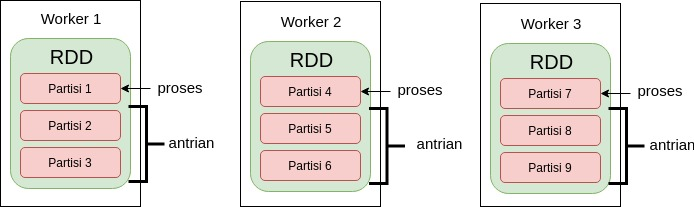
\includegraphics[scale=0.6]{workerprocess}  
    \caption[\textit{Worker} memproses partisi]{\textit{Worker} memproses partisi} 
    \label{fig:workerprocess} 
\end{figure}

\item Hasil dari tahap \textit{map} akan dilanjutkan kepada \textit{reducer}. Pada tahap ini \textit{reducer} akan memanggil metode \textit{agglomerative clustering} untuk mereduksi keluaran dari \textit{mapper} seperti pada Gambar \ref{fig:reducespark}. Pada tahap \textit{reducer}, akan dibangun \textit{dendrogram} menggunakan algoritma HAC. \textit{Dendrogram} akan dipotong untuk menghasilkan \textit{clusters}. Setiap cluster akan dicari polanya, pola ini akan dikembalikan sebagai hasilnya.

\begin{figure}[H]
    \centering  
    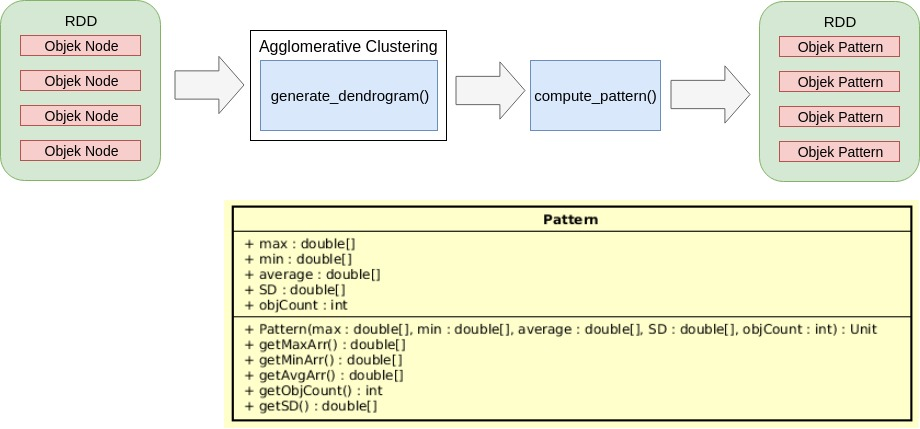
\includegraphics[scale=0.5]{reducespark}  
    \caption[Proses reduksi pada \textit{reducer} dan kelas \textit{Pattern}]{Proses reduksi pada \textit{reducer} dan kelas \textit{Pattern}} 
    \label{fig:reducespark} 
\end{figure}


\item Terakhir, pola dari hasil \textit{reduce} akan disimpan pada HDFS. Bila semua partisi sudah diproses, perangkat lunak akan berhenti. Bila masih ada partisi yang tersisa, langkah 3, 4 dan 5 akan diulang kembali sampai semua partisi telah diproses.

\begin{figure}[H]
    \centering  
    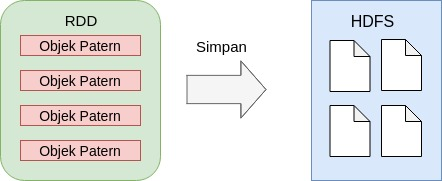
\includegraphics[scale=0.5]{savehdfs}  
    \caption[Penyimpanan pola pada HDFS]{Penyimpanan pola pada HDFS} 
    \label{fig:savehdfs} 
\end{figure}

\end{enumerate}

\subsection{Analisis Hierarchical Agglomerative Clustering untuk Spark}

Setelah mempelajari algoritma \textit{Hierarchical Agglomerative Clustering} pada MapReduce, \textit{format} masukan yang harus diproses dan keluaran yang harus dihasilkan, berikut adalah penjelasan \textit{pseudocode} algoritma \textit{map} dan \textit{reduce} untuk Spark:\\

\begin{algorithm}[H]
	\label{alg:map}
	\DontPrintSemicolon\SetAlgoNoLine\LinesNumbered
	\SetKwInOut{Input}{Masukan}
	\SetKwInOut{Output}{Keluaran}
	\SetKwInOut{Desc}{Deskripsi}
	\Input{dataset ($D$) bertipe RDD[String]}
	\Output{$DN$ = dataset baru bertipe RDD[Node]}
	\Desc{Melakukan \textit{parsing} untuk setiap elemen pada RDD $D$ dan mengembalikan RDD baru bertipe Node  }
	\SetKwHangingKw{DN}{\textbf{\textit{DN}} $\leftarrow$}
	\SetKwHangingKw{node}{\textbf{\textit{node}} $\leftarrow$}
	\SetKwHangingKw{split}{\textbf{\textit{split}} $\leftarrow$}
	\BlankLine
	\Begin{
		\DN{RDD bertipe Node yang kosong}
		\ForEach{line pada \textbf{\textit{D}}}{
			\node{node baru}
			\split{split \textit{line} berdasarkan delimeter "," dan konversi menjadi double}
			node.setData(\textbf{\textit{split}})\;
			\DN{\textbf{\textit{DN}} join \textbf{\textit{node}}}
		}
		return \textbf{\textit{DN}}
	}
	
	\caption{Algoritma \textit{Map}}
	
\end{algorithm}

\clearpage

\begin{algorithm}[H]
	\label{alg:reduce}
	\DontPrintSemicolon\SetAlgoNoLine\LinesNumbered
	\SetKwInOut{Input}{Masukan}
	\SetKwInOut{Desc}{Deskripsi}
	\Input{($DN$) RDD[Node] hasil dari mapper, jumlah objek maksimum ($MX$), tipe metode yang dipakai ($distType$) $\epsilon$ \{\textit{single}, \textit{complete}, \textit{centroid}\}, dan \textit{cut-off distance} ($co$) }
	\Desc{Membuat \textit{dendrogram} dari hasil \textit{map} sesuai dengan batasan yang diberikan, membatasi jumlah objek yang akan diolah menjadi \textit{dendrogram} berdasarkan \textit{MX}, memotong dendrogram bersadarkan nilai $co$, mendapatkan pola \textit{pt} dari potongan \textit{cluster}, menyimpan pola-pola pada HDFS}
	\SetKwHangingKw{isP}{\textbf{\textit{isProcessed}} $\leftarrow$}
	\SetKwHangingKw{objL}{\textbf{\textit{objectList}} $\leftarrow$}
	\SetKwHangingKw{rdp}{\textbf{\textit{patterns}} $\leftarrow$}
	\SetKwHangingKw{dendo}{\textbf{\textit{dendrogram}} $\leftarrow$}
	\SetKwHangingKw{pt}{\textbf{\textit{pt}} $\leftarrow$}

	\BlankLine
	\Begin{
		\textit{broadcast} nilai $MX$, $distType$, dan $co$ \;
		\objL{[] array Node kosong}
		\rdp{RDD bertipe Pattern untuk mengumpulkan pola hasil reduksi}
		\ForEach{elemen in \textbf{DN}} {
			\objL{objectList join \textit{elemen}}
			\isP{false}
			\If{count(objectList) == \textit{MX}}{
				\dendo{generate\_dendrogram(\textbf{\textit{\textbf{objectList}, $distType$}})}
				\pt{compute\_pattern(dendrogram,$co$)}
				\rdp{\textbf{\textit{pattern}} join \textit{\textbf{pt}}}
				\isP{true}
				kosongkan \textbf{\textit{objectList}}\;
			}
		}
		\If{isProcessed == false}{
			\dendo{\textit{generate\_dendrogram}(\textbf{\textit{\textbf{objectList}, $distType$}})}
			\pt{\textit{compute\_pattern}(dendrogram,$co$)}
			\rdp{\textbf{\textit{pattern}} join \textit{\textbf{pt}}}

		}
		\ForEach{pattern in \textbf{patterns}}{
			simpan pattern pada HDFS
		}
		
	}
	
	\caption{Algoritma \textit{Reduce}}
	
\end{algorithm}

\clearpage

\RestyleAlgo{boxed}
\begin{algorithm}[H]
	\label{alg:hac}
	\SetKwFunction{FMain}{generate\_dendrogram}
  	\SetKwProg{Fn}{Function}{:}{}
	\DontPrintSemicolon\SetAlgoNoLine\LinesNumbered
	\Fn{\FMain{$objectList$, $distType$}}{
		\SetKwInOut{Input}{Masukan}
		\SetKwInOut{Output}{Keluaran}
		\SetKwInOut{Desc}{Deskripsi}
		\Input{list objek-objek $objectList$, tipe metode $distType$}
		\Output{dendrogram}
		\Desc{Membangun \textit{dendrogram} dari list objek sesuai dengan nilai $distType$ yang diberikan }
		\BlankLine
  		\Begin{	
        	distanceMatrix[][]\;
			dendrogram[]\;
			inisialisasi distranceMatrix dan dendrogram\;
			\While{dendrogram.length != 1}{
				gabungkan objek terdekat berdasarkan nilai pada distanceMatrix\;
				perbarui dendrogram\;
				hitung kembali distanceMatrix berdasarkan $distType$\;
			}
			return dendrogram[0]
 		}
 	}
	
\end{algorithm}

\clearpage

\RestyleAlgo{boxed}
\begin{algorithm}[H]
	\label{alg:patern}
	\SetKwFunction{FMain}{compute\_pattern}
  	\SetKwProg{Fn}{Function}{:}{}
	\DontPrintSemicolon\SetAlgoNoLine\LinesNumbered
	\Fn{\FMain{$dendrogram$, $co$}}{
		\SetKwInOut{Input}{Masukan}
		\SetKwInOut{Output}{Keluaran}
		\SetKwInOut{Desc}{Deskripsi}
		\Input{$dendrogram$, \textit{cut-off distance} $co$}
		\Output{pola-pola dari seluruh potongan cluster}	
		\Desc{Memotong \textit{dendrogram} menjadi beberapa \textit{clusters} berdasarkan nilai $co$, mendapatkan pola dari setiap \textit{cluster}}
		\SetKwHangingKw{dist}{\textbf{\textit{dist}} $\leftarrow$}
		\SetKwHangingKw{node}{\textbf{\textit{node}} $\leftarrow$}
		\SetKwHangingKw{le}{\textbf{\textit{left}} $\leftarrow$}
		\SetKwHangingKw{ri}{\textbf{\textit{right}} $\leftarrow$}
		\SetKwHangingKw{pat}{\textbf{\textit{p}} $\leftarrow$}
		\BlankLine
  		\Begin{	
        	bfs[] \\ array kosong bertipe Node\;
        	clusters[] \\ array kosong untuk menyimpan hasil potongan dari dendrogram\;
        	bfs.add($dendrogram$)\;
        	\dist{$co$ * $dendrogram$.distance}
        	\While{bfs tidak kosong}{
        		\node{bfs.remove(0)}
        		\eIf{\textbf{\textit{node}}.distance <= dist}{
        			clusters.add(\textbf{\textit{node}})\;
        		}{
        			\le{\textbf{\textit{node}}.left}
        			\ri{\textbf{\textit{node}}.right}
        			\If{\textbf{\textit{left}} != null}{
        				bfs.add(\textbf{\textit{left}})\;
        			}
        			\If{\textbf{\textit{right}} != null}{
        				bfs.add(\textbf{\textit{right}})\;
        			}
        		}
        	}
        	patterns[]\;
        	\ForEach{cluster in clusters}{
        		\pat{dapatkan pola dari setiap \textit{cluster}}
        		patterns.add(\textbf{\textit{p}})\;
        	}
        	return patterns
 		}
 	}
	
\end{algorithm}
 
Algoritma \textit{Map} ~\ref{alg:map} ini bertujuan untuk melakukan \textit{parsing} terhadap masukan yang diberikan. Masukan yang masuk berupa RDD[String] akan di-\textit{parsing} menjad RDD[Node]. Pertama, elemen pada RDD[String] yang berupa \textit{String} akan di pecah berdasarkan \textit{delimeter} "," dan di konversi menjadi bilangan pecahan. Hasilnya merupakan \textit{array} bertipe \textit{double} yang menjadi atribut objek \textit{Node}. Objek \textit{Node} kemudian akan tambahkan kepada RDD[Node]. RDD[Node] akan dikembalikan sebagai hasil untuk tahap \textit{reduce}.\\

Algoritma \textit{Reduce} ~\ref{alg:reduce} bertujuan untuk membangun dendrogram dan mengembalikan pola-pola bertipe RDD[Pattern] sebagai hasilnya. Pertama-tama nilai $MX$, $distType$, $co$ akan di \textit{broadcast} agar setiap \textit{worker} memiliki nilai tersebut. \textit{Variable} \textit{objectList} dibuat untuk menampung \textit{Node-Node} yang akan dibangun menjadi \textit{dendrogram}. \textit{Node} pada RDD[Node] akan ditambahkan kepada \textit{objectList} sampai batas jumlah \textit{Node} pada objectList sama dengan nilai $MX$. Kemudian, fungsi \textit{generate\_dendrogram(objectList, distType)} akan dipanggil untuk membangun dendrogram. Hasil dari fungsi tersebut yaitu sebuah \textit{dendrogram} dijadikan masukan untuk fungsi \textit{compute\_pattern(dendrogram,co)}. Fungsi ini untuk memotong dendrogram menjadi \textit{clusters} dan mencari pola dari setiap \textit{cluster}. Pola atau \textit{Pattern} akan ditambahkan kepada \textit{variable pattern} (RDD[Pattern]) yang akan dikembalikan sebagi hasil. \textit{variable isProcessed} pada baris 16 untuk memastikan bahwa setiap elemen pada \textit{objectList} sudah di proses. \\


Fungsi \textit{generate}\_\textit{dendrogram} pada algoritma ~\ref{alg:reduce} digunakan untuk membangun \textit{dendrogram}. Fungsi ini akan menerima \textit{objectList} sebagai masukan. Pertama-tama \textit{array} distanceMatrix harus diinisialisasi dan dihitung jarak antara objeknya menggunakan \textit{distType} yang ditentukan. Kemudian, \textit{array} \textit{dendrogram} diisi dengan objek-objek pada \textit{objectList}. Untuk membangun dendrogram, gabungkan objek yang memiliki nilai terkecil pada \textit{distanceMatrix} seperti pada Gambar ~\ref{fig:hac}. Setelah menggabungkan dua buah objek, objek pada dendrogram akan berkurang 1 dan \textit{distranceMatrix} harus dihitung ulang berdasarkan \textit{distType}.

\begin{figure}[H]
    \centering  
    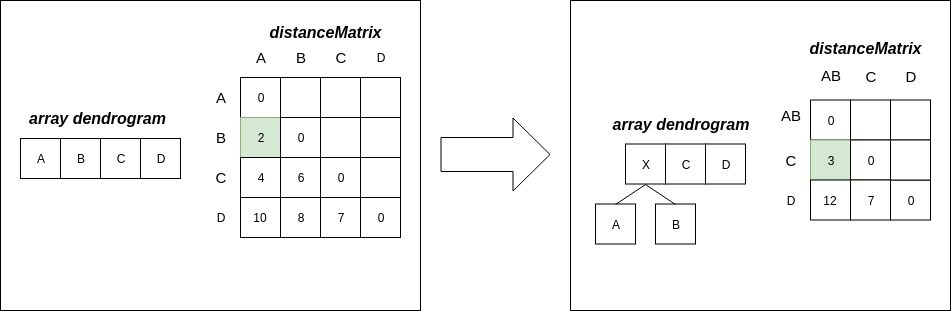
\includegraphics[scale=0.5]{hac}  
    \caption[Contoh perhitungan matriks dan pembentukan dendrogram]{Contoh perhitungan matriks dan pembentukan dendrogram} 
    \label{fig:hac}
\end{figure}

Fungsi \textit{compute}\_\textit{pattern} pada algoritma ~\ref{alg:reduce} digunakan untuk mendapatkan pola dari \textit{cluster}. Fungsi ini menerima hasil \textit{dendrogram} dari fungsi \textit{generate}\_\textit{dendrogram}, berserta nilai \textit{cut-off distance} sebagai masukannya. Pertama-tama \textit{dendrogram} yang diwakili dengan struktur \textit{tree} akan ditelusuri di setiap tingkatnya. Jarak pada setiap tingkat akan di cek. Bila jarak sudah kurang dari jarak hasil perkalian $co$ dengan tinggi \textit{dendrogram}, maka \textit{dendrogram} akan dipotong untuk menghasilkan potongan \textit{clusters}. Setelah itu, pola dari setiap cluster akan dicari. Pola didapatkan dengan mencari nilai minimum, maksimum, rata-rata dan standard deviasi dari setiap attribute pada \textit{cluster}. Pola akan dikembalikan sebagai hasil.

\begin{figure}[H]
    \centering  
    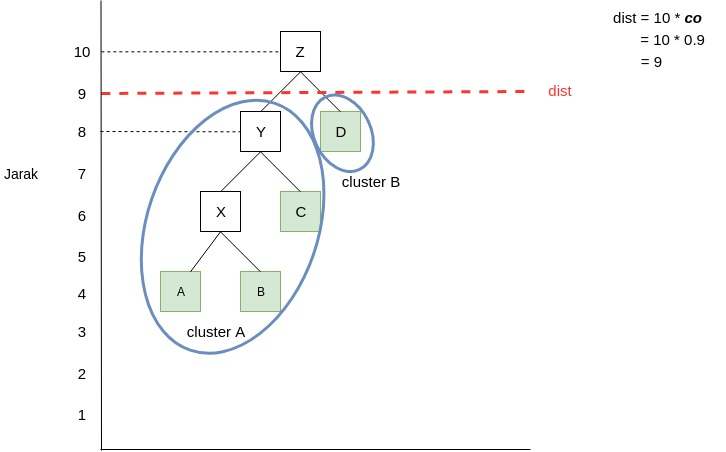
\includegraphics[scale=0.6]{tree}  
    \caption[Contoh pemotongan \textit{dendrogram}]{Contoh pemotongan \textit{dendrogram}} 
    \label{fig:tree} 
\end{figure}


 

\section{Perancangan Perangkat Lunak}

Pada bagian ini, akan dijelaskan perancangan perangkat lunak.  Perancangan termasuk diagram \textit{use case}, skenario, diagram kelas, dan rancangan antarmuka. 


\subsection{Diagram Use Case dan Skenario}

Diagram \textit{use case} merupakan sebuah pemodelan untuk perilaku dari perangkat lunak yang akan dibuat. Diagram \textit{use case} digunakan untuk mengetahui fungsi apa saja yang ada dalam perangkat lunak. Fungsi-fungsi dari perangkat lunak akan dioperasikan oleh satu pengguna. Cara kerja dan perilaku dari perangkat lunak akan dijelaskan dalam bentuk diagram \textit{use case}. Diagram \textit{use case} dapat dilihat pada Gambar ~\ref{fig:usecase}.

\begin{figure}[H]
    \centering  
    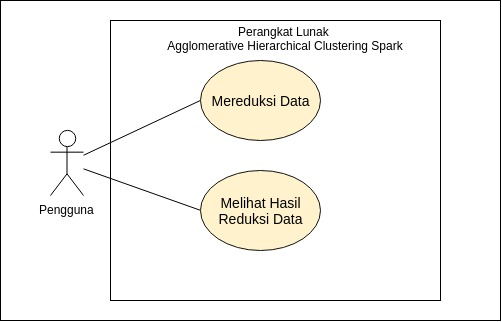
\includegraphics[scale=0.7]{usecase}  
    \caption[Diagram \textit{use case} perangkat lunak \textit{Hierarchical Agglomerative Clustering}]{Diagram \textit{use case} perangkat lunak \textit{Hierarchical Agglomerative Clustering}} 
    \label{fig:usecase} 
\end{figure}

Berdasarkan gambar diagram \textit{use case} diatas, berikut adalah skenario yang ada:

\begin{enumerate}

\item Nama \textit{use case}: Mereduksi data

\begin{itemize}
\item Aktor: Pengguna

\item Pre-kondisi: data yang akan diolah dimasukan kepada HDFS.

\item Pra-kondisi: hasil reduksi disimpan pada HDFS.

\item Deskripsi: Fitur untuk menjalankan program untuk mereduksi data.

\item Langkah-langkah:

\begin{enumerate}

\item Pengguna mengisi JAR \textit{path}, \textit{input path}, dan \textit{output path}.

\item Pengguna mengisi jumlah \textit{executor} dan besar \textit{executor memory}.

\item Pengguna mengisi jumlah partisi, batas maksimum objek, tipe metode, dan \textit{cut-off distance}. 

\item Pengguna menekan tombol \textit{submit}.

\item Sistem melakukan pengolahan data dengan algoritma \textit{Hierarchical Agglomerative Clustering} pada \textit{cluster} Hadoop.

\item Sistem membuka halaman baru untuk melihat tahap dan progres program.

\item Sistem menyimpan hasil reduksi pada HDFS.
\end{enumerate}

\end{itemize}


\item Nama \textit{use case}: Mengunduh data

\begin{itemize}
\item Aktor: Pengguna

\item Pre-kondisi: data yang akan diunduh sudah disimpan pada HDFS.

\item Pra-kondisi: data dapat diunduh dari HDFS.

\item Deskripsi: fitur untuk mengunduh data hasil reduksi.

\item Langkah-langkah:

\begin{enumerate}

\item Pengguna mengisi \textit{path} dimana data disimpan pada HDFS.

\item Sistem membuka halaman baru dimana pengguna dapat mengunduh data dari HDFS .

\end{enumerate}

\end{itemize}

\end{enumerate}


\subsection{Diagram Kelas}

Pada bagian ini akan dijelaskan diagram kelas dari perangkat lunak. Diagram kelas dapat dilihat pada Gambar ~\ref{fig:classdiagram}.

\begin{figure}[H]
    \centering  
    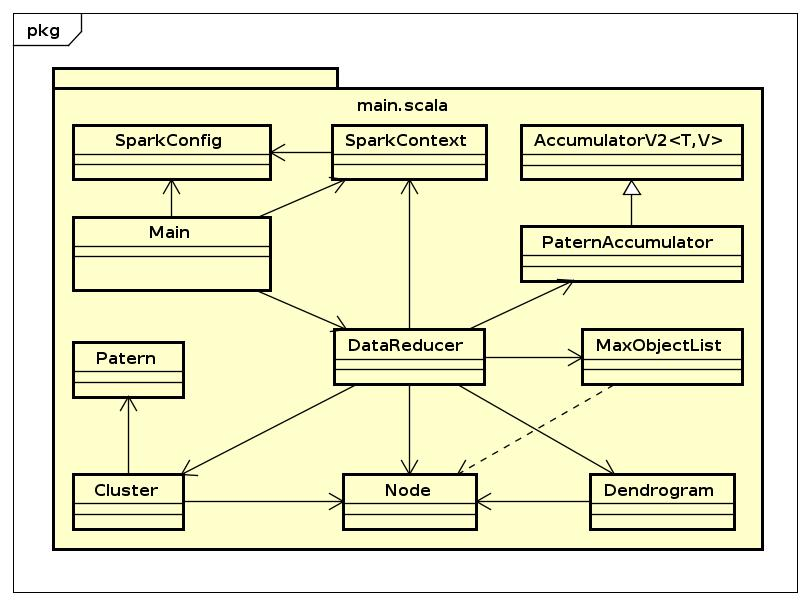
\includegraphics[scale=0.5]{classdiagram}  
    \caption[Diagram kelas]{Diagram kelas} 
    \label{fig:classdiagram} 
\end{figure}

Berdasarkan Gambar ~\ref{fig:classdiagram}, berikut ini adalah penjelasan kelas-kelas yang digunakan:

\begin{itemize}

\item \textbf{Main, Spark Config, dan Spark Context}\\

\begin{figure}[H]
    \centering  
    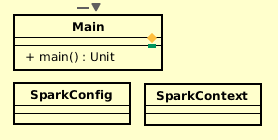
\includegraphics[scale=0.75]{maindiagram}  
    \caption[Kelas Main, SparkConfig, SparkContext]{Kelas Main, SparkConfig, SparkContext} 
    \label{fig:maindiagram} 
\end{figure}

Berikut adalah penjelasan dari ketiga kelas pada Gambar ~\ref{fig:maindiagram}:

\begin{itemize}

\item \textit{Main}: kelas \textit{Main} memiliki \textit{method main}  yang merupakan titik masuk dari program. \textit{Method} ini merupakan \textit{method} pertama yang akan dieksekusi ketika program dijalankan.

\item \textit{SparkConfig}: kelas \textit{SparkConfig} digunakan untuk mengatur konfigurasi untuk Spark. Pengaturan nama aplikasi, jumlah \textit{core}, besar \textit{memory}, dan lainya dapat diatur pada kelas ini.

\item \textit{SparkContext}: kelas ini merupakan titik masuk untuk layanan-layan dari Apache Spark.\\

\end{itemize}


\item \textbf{DataReducer}\\

\begin{figure}[H]
    \centering  
    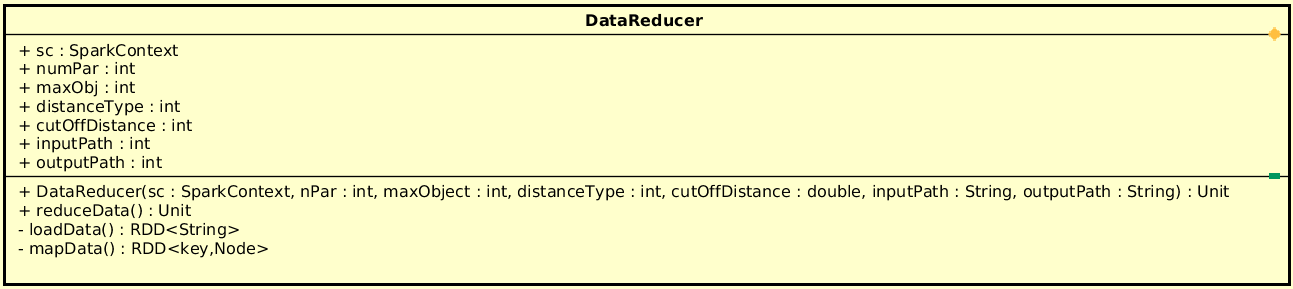
\includegraphics[scale=0.5]{datareducer}  
    \caption[Kelas DataReducer]{Kelas DataReducer} 
    \label{fig:datareducer} 
\end{figure}

Kelas \textit{DataReducer} dirancang untuk memproses data. Proses reduksi secara parallel dilakukan pada kelas ini. Proses pemuatan dan penyimpanan data dilakukan pada kelas ini. Berdasarkan Gambar ~\ref{fig:datareducer}, berikut adalah penjelasan dari \textit{methods} pada kelas DataReducer:

\begin{itemize}

\item \textit{loadData}: \textit{method} untuk memuat data berdasarkan \textit{input path} yang diberikan.

\item \textit{mapData}: \textit{method} untuk mengubah baris-baris attribut bertipe \textit{String} menjadi objek Node. \textit{Method} ini akan mengembalikan RDD bertipe Node.  

\item  \textit{reduceData}: \textit{method} untuk mereduksi data menggunakan \textit{agglomerative clustering}. Method ini akan mengembalikan pola-pola dari setiap \textit{clusters}.\\

\end{itemize}


\item \textbf{Dendrogram}\\

\begin{figure}[H]
    \centering  
    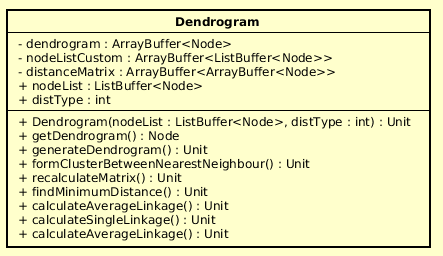
\includegraphics[scale=0.6]{dendrogramdiagram}  
    \caption[Kelas Dendrogram]{Kelas Dendrogram} 
    \label{fig:dendrogramdiagram} 
\end{figure}

Kelas \textit{Dendrogram} dirancang untuk memproses data dan membangun \textit{dendrogram} sesuai algoritma \textit{Hierarchical Agglomerative Clustering}. Berdasarkan Gambar ~\ref{fig:dendrogramdiagram}, berikut adalah penjelasan \textit{methods} pada kelas \textit{Dendrogram}:

\begin{itemize}
\item \textit{getDendrogram}: \textit{method} ini mengembalikan \textit{dendrogram}.

\item \textit{generateDendrogram}: \textit{Method} untuk membangun \textit{dendrogram} berdasarkan algoritma \textit{Hierarchical Agglomerative Clustering}. 

\item \textit{formClusterBetweenNearestNeighbour}: method untuk menggabungkan \textit{cluster} terdekat.

\item \textit{recalculateMatrix}: \textit{method} untuk menghitung ulang matriks jarak.

\item \textit{findMinimumDistance}: \textit{method} untuk mencari jarak minimum antara dua \textit{cluster}.

\item \textit{calculateCentroidLinkage}: \textit{method} untuk mencari jarak antara \textit{centorid} dua buah \textit{cluster}.

\item \textit{calculateSingleLinkage}: \textit{method} untuk mencari jarak minimum antara dua buah \textit{cluster}.

\item \textit{calculateCompleteLinkage}: \textit{method} untuk mencari jarak maksimum antara dua \textit{cluster}.

\item \textit{calculateDistance}: \textit{method} untuk mencari jarak antara dua buah \textit{Node} berdasarkan atributnya.\\
 
\end{itemize}


\item \textbf{Cluster}\\

\begin{figure}[H]
    \centering  
    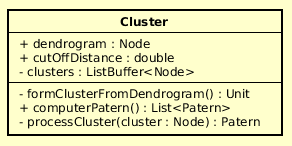
\includegraphics[scale=0.6]{clusterdiagram}  
    \caption[Kelas Cluster]{Kelas Cluster} 
    \label{fig:clusterdiagram} 
\end{figure}

Kelas \textit{Cluster} dirancang untuk mengolah \textit{cluster} untuk menghasilkan pola dengan memotong \textit{cluster}. Berdasarkan Gambar ~\ref{fig:clusterdiagram}, berikut adalah penjelasan \textit{methods} pada kelas \textit{Cluster}:

\begin{itemize}

\item \textit{formClusterFromDendrogram}: method ini bertugas untuk memotong \textit{dendrogram} menjadi beberapa \textit{cluster}.

\item \textit{computePattern}: method untuk mengolah potongan-potongan \textit{cluster} menjadi pola dengan memanggil \textit{method} processCluster.

\item \textit{processCluster}: method untuk memproses \textit{cluster} dan membuat pola berdasarkan anggota-anggota pada \textit{cluster}.\\
 
\end{itemize}


\item \textbf{Pattern}\\

\begin{figure}[H]
    \centering  
    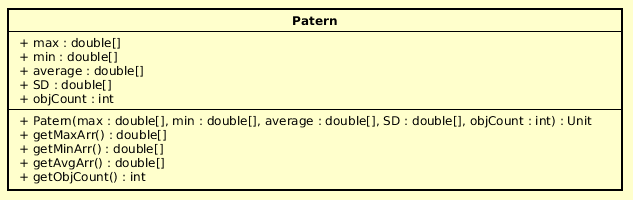
\includegraphics[scale=0.6]{paterndiagram}  
    \caption[Kelas Pattern]{Kelas Pattern} 
    \label{fig:paterndiagram} 
\end{figure}

Kelas \textit{Patern} dirancang untuk merepresentasikan pola pada \textit{cluster}. Berdasarkan Gambar ~\ref{fig:clusterdiagram}, berikut adalah penjelasan \textit{methods} pada kelas \textit{Pattern}:

\begin{itemize}

\item \textit{getMaxArr}: \textit{method} ini mengembalikan \textit{array} berisi nilai maksimum dari setiap atribut.

\item \textit{getMinArr}: \textit{method} ini mengembalikan \textit{array} berisi nilai minimum dari setiap atribut.

\item \textit{getAvgArr}: \textit{method} ini mengembalikan \textit{array} berisi nilai rata-rata dari setiap atribut.

\item \textit{getSDArr}: \textit{method} ini mengembalikan \textit{array} berisi nilai standar deviasi dari setiap atribut.

\item \textit{getObjCount}: \textit{method} ini mengembalikan jumlah objek.\\
 
\end{itemize}


\item \textbf{Node}\\

\begin{figure}[H]
    \centering  
    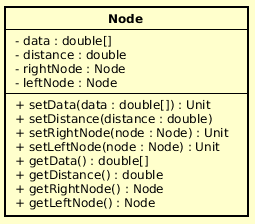
\includegraphics[scale=0.6]{nodediagram}  
    \caption[Kelas Node]{Kelas Node} 
    \label{fig:nodediagram} 
\end{figure}

Kelas \textit{Node} digunakan untuk membentuk pohon yang merepresentasikan \textit{dendrogram}. Selain itu kelas ini digunakan untuk merepresentasikan anggota pada \textit{cluster}.  Berdasarkan Gambar ~\ref{fig:nodediagram}, berikut adalah penjelasan \textit{methods} pada kelas \textit{Node}:

\begin{itemize}

\item \textit{setData}: \textit{method} untuk memasukan nilai-nilai atribut.

\item \textit{setDistance}: \textit{method} untuk megubah nilai jarak.

\item \textit{setRightNode}: \textit{method} untuk menambahkan anak kanan \textit{Node}.

\item \textit{setLeftNode}: \textit{method} untuk menambahkan anak kiri \textit{Node}.

\item \textit{getData}: \textit{method} ini mengembalikan nilai-nilai atribut.

\item \textit{getDistance}: \textit{method} ini mengembalikan jarak.

\item \textit{getRightNode}: \textit{method} ini mengebalikan anak belah kanan dari \textit{Node}.

\item \textit{getLeftNode}: \textit{method} ini mengebalikan anak belah kiri dari \textit{Node}.

\end{itemize}


\end{itemize}


\subsection{Rancangan Antarmuka}

Antarmuka dirancang untuk mempermudah pengguna dalam menjalankan program dan mengambil hasil data yang telah direduksi. Ada dua buah menu utama yang dapat dipilih oleh pengguna, menu \textit{Submit} dan \textit{Data}. Menu \textit{Submit} digunakan untuk menjalankan aplikasi dan menu \textit{Data} digunakan untuk mengunduh data hasil reduksi. Berikut adalah penjelasan rancangan antaramuka:

\begin{enumerate}

\item Perancangan halaman \textit{Submit} untuk mempermudah penggunan menjalankan aplikasi. Pada halaman ini, disediakan \textit{form} bereserta \textit{input parameter} yang dibutuhkan untuk menjalankan aplikasi. Gambar rancangan antarmuka dapat dilihat pada Gambar ~\ref{fig:antarmuka1}

\begin{figure}[H]
    \centering  
    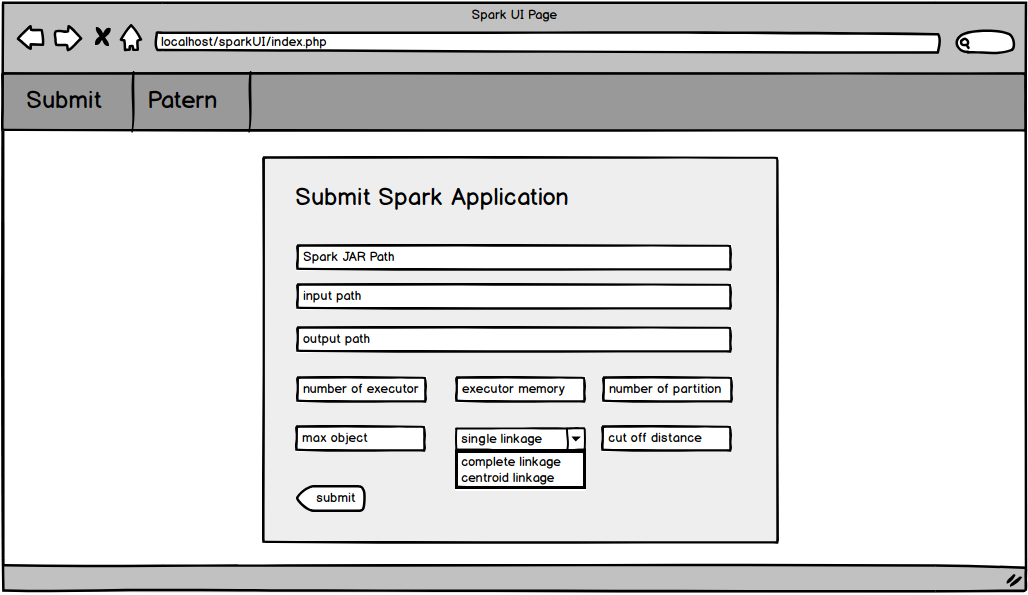
\includegraphics[scale=0.42]{antarmuka1}  
    \caption[Recangan antaramuka menu \textit{submit}]{Rancangan antaramuka menu \textit{submit}} 
    \label{fig:antarmuka1} 
\end{figure}

Berdasarkan Gambar ~\ref{fig:antarmuka1}, berikut adalah penjelasan \textit{input field} yang ada:

\begin{itemize}
\item \textit{Spark JAR Path}: \textit{field} untuk direktori JAR.

\item \textit{input path}: \textit{field} untuk direktori file \textit{input} pada HDFS.

\item \textit{output path}: \textit{field} untuk direktori tempat penyimpanan hasil pada HDFS.

\item \textit{number of executor}: \textit{field} untuk menentukan jumlah \textit{executor} yang akan dipakai.

\item \textit{executor memory}: \textit{field} untuk menentukan jumlah memori yang akan dipakai.

\item \textit{number of partition}: \textit{field} untuk menentukan jumlah partisi untuk data.

\item \textit{max object}: \textit{field} untuk membatasi jumlah objek pada yang akan diolah.

\item \textit{drop down} (\textit{single linkage}, \textit{comlete linkage}, \textit{centroid linkage}): kotak pilihan untuk memilih  metode \textit{single linkage}, \textit{complete linkage} atau \textit{centroid linkage} yang digunakan untuk memproses data.

\item \textit{cut off distance}: \textit{field} untuk menentukan jarak untuk memotong \textit{dendrogram} menjadi \textit{clusters}.

\end{itemize} 

Setelah pengguna menekan tombol \textit{submit} pada \textit{form}, pengguna akan dipindakan ke halaman baru seperti pada Gambar ~\ref{fig:antarmukaresult}. Selain itu, halaman \textit{Hadoop web UI} akan terbuka di tab baru seperti pada Gambar ~\ref{fig:hadoopweb}.

\begin{figure}[H]
    \centering  
    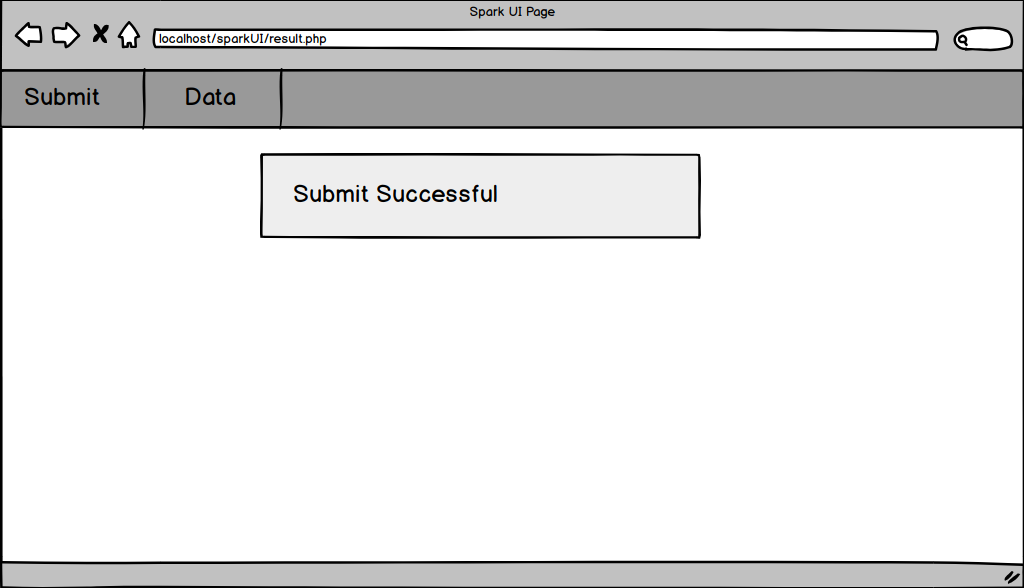
\includegraphics[scale=0.42]{antarmukaresult}  
    \caption[Rancangan antaramuka \textit{result}]{Rancangan antaramuka halaman \textit{result}} 
    \label{fig:antarmukaresult} 
\end{figure}

\begin{figure}[H]
    \centering  
    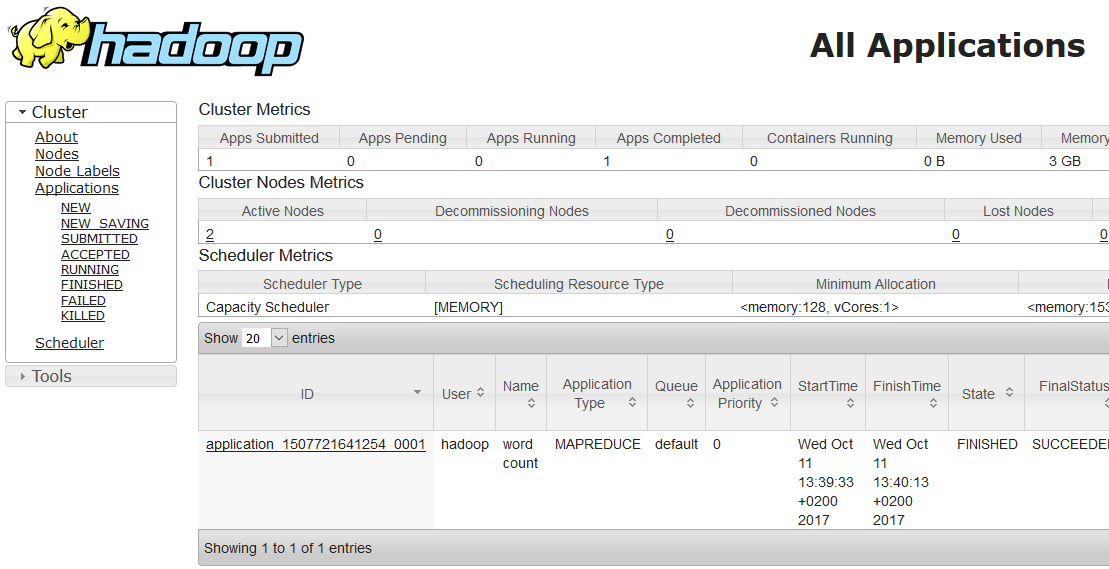
\includegraphics[scale=0.4]{hadoopweb}  
    \caption[Halaman web Hadoop]{Halaman web Hadoop} 
    \label{fig:hadoopweb} 
\end{figure}


\item Perancangan halaman antarmuka menu \textit{Data} (Gambar ~\ref{fig:antarmuka2}) digunakan untuk membuka diretori dimana data disimpan pada HDFS. Ketika pengguna memasukan direktori, pengguna akan dipindahkan ke dalaman baru (Gambar ~\ref{fig:antarmuka3}) dan sebuah halaman (Gambar ~\ref{fig:hdfsweb}) akan dibuka untuk menampilkan data yang bisa diunduh. Ketika pengguna menetkan salah satu nama file pada halaman \textit{list} (\ref{fig:antarmuka3}), pengguna dapat melihat isi dari data yang ada dari file tersebut di halaman (\ref{fig:antarmuka4}).  

\begin{figure}[H]
    \centering  
    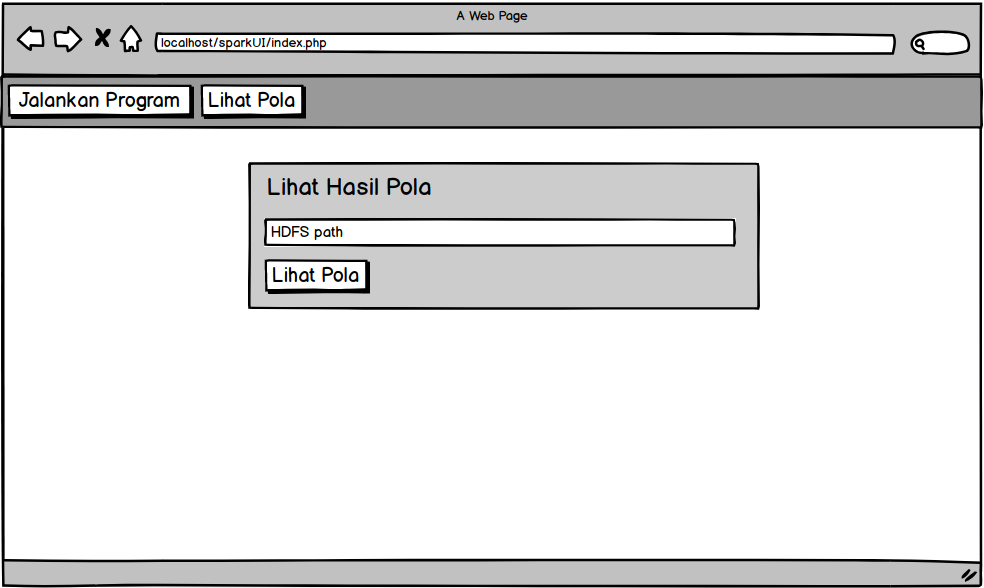
\includegraphics[scale=0.42]{antarmuka2}  
    \caption[Rancangan antarmuka menu \textit{Data}]{Rancangan antarmuka menu \textit{Data}} 
    \label{fig:antarmuka2} 
\end{figure}

\begin{figure}[H]
    \centering  
    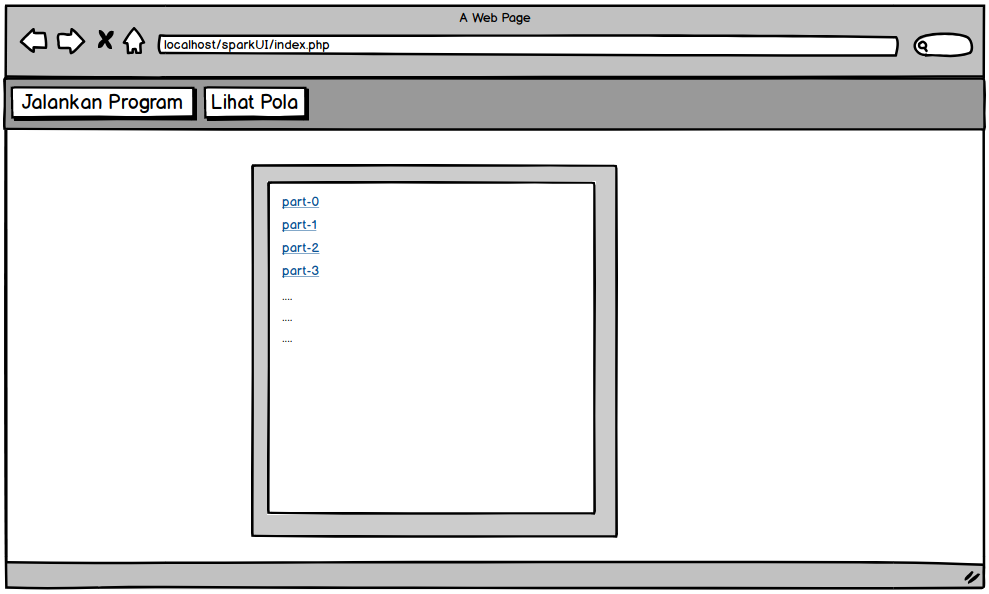
\includegraphics[scale=0.42]{antarmuka3}  
    \caption[Rancangan antarmuka halaman \textit{list}]{Rancangan antarmuka halaman \textit{list}} 
    \label{fig:antarmuka3} 
\end{figure}

\begin{figure}[H]
    \centering  
    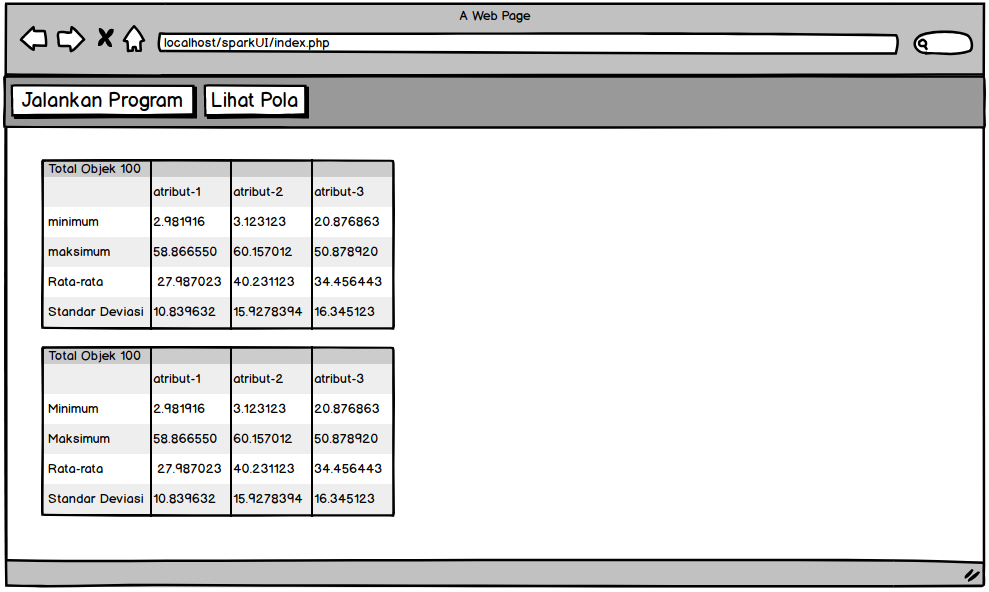
\includegraphics[scale=0.42]{antarmuka4}  
    \caption[Rancangan antarmuka halaman data]{Rancangan antarmuka halaman data} 
    \label{fig:antarmuka4} 
\end{figure}

\begin{figure}[H]
    \centering  
    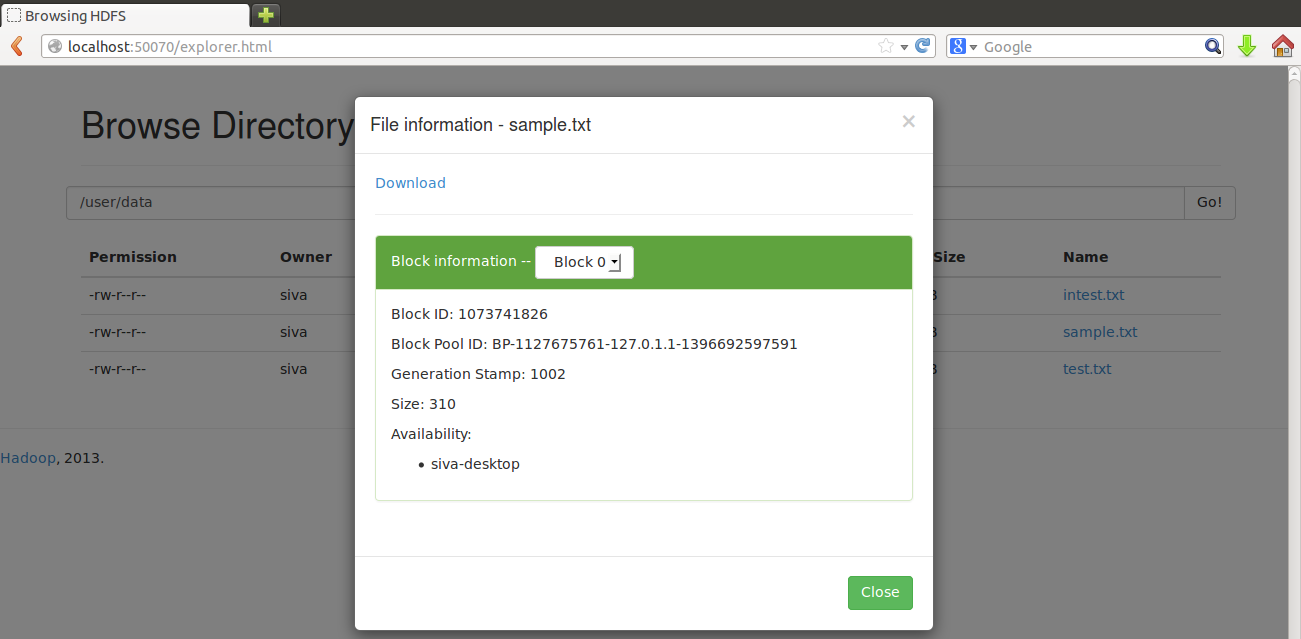
\includegraphics[scale=0.35]{hdfsweb}  
    \caption[Halaman web HDFS]{Halaman web HDFS} 
    \label{fig:hdfsweb} 
\end{figure}


\end{enumerate}



